% -*- latex -*-
%%%%%%%%%%%%%%%%%%%%%%%%%%%%%%%%%%%%%%%%%%%%%%%%%%%%%%%%%%%%%%%%
%%%%
%%%% This TeX file is part of the tutorial
%%%% `Introduction to the PETSc library'
%%%% Victor Eijkhout, eijkhout@tacc.utexas.edu
%%%% copyright Victor Eijkhout 2012-2020
%%%%
%%%%%%%%%%%%%%%%%%%%%%%%%%%%%%%%%%%%%%%%%%%%%%%%%%%%%%%%%%%%%%%%

\sectionframe{\texttt{KSP \& PC}: Iterative solvers}

\frame{\frametitle{What are iterative solvers?}

Solving a linear system $Ax=b$ with Gaussian elimination can take lots
of time/memory.

Alternative: iterative solvers use successive approximations of the
solution:
\begin{itemize}
\item Convergence not always guaranteed
\item Possibly much faster / less memory
\item Basic operation: $y\leftarrow Ax$ executed once per iteration
\item Also needed: preconditioner $B\approx A^{-1}$
\end{itemize}
}

\frame[containsverbatim]{\frametitle{Topics}
  \begin{itemize}
  \item All linear solvers in PETSc are iterative, even the direct ones
  \item Preconditioners
  \item Fargoing control through commandline options
  \item Tolerances, convergence and divergence reason
  \item Custom monitors and convergence tests
  \end{itemize}
}

%\subsectionframe{KSP: Krylov Space objects}

\frame[containsverbatim]{\frametitle{Iterative solver basics}
\begin{verbatim}
KSPCreate(comm,&solver); KSPDestroy(solver);
// set Amat and Pmat
KSPSetOperators(solver,A,B); // usually: A,A
// solve
KSPSolve(solver,rhs,sol);
\end{verbatim}
Optional: \n{KSPSetup(solver)}

Reuse \n{Amat} or \n{Pmat}: \n{KSPGetOperators} and \n{PetscObjectReference}.
}

\frame[containsverbatim]{\frametitle{Solver type}

\begin{verbatim}
KSPSetType(solver,KSPGMRES);
\end{verbatim}

KSP can be controlled from the commandline:
\begin{verbatim}
KSPSetFromOptions(solver);
/* right before KSPSolve or KSPSetUp */
\end{verbatim}
then options \n{-ksp....} are parsed.
\begin{itemize}
\item type: \n{-ksp_type gmres -ksp_gmres_restart 20}
\item \n{-ksp_view}
\end{itemize}

}

\frame[containsverbatim]{\frametitle{Convergence}
Iterative solvers can fail
  \begin{itemize}
  \item Solve call itself gives no feedback: solution may be completely wrong
  \item \n{KSPGetConvergedReason(solver,&reason)} : \\
    positive is convergence, negative divergence \\
    \n{KSPConvergedReasons[reason]} is string      
  \item \n{KSPGetIterationNumber(solver,&nits)} : after how many
    iterations did the method stop?
  \end{itemize}
}

\frame[containsverbatim]{
\begin{verbatim}
KSPSolve(solver,B,X);
KSPGetConvergedReason(solver,&reason);
if (reason<0) {
  PetscPrintf(comm,
    "Failure to converge after %d iterations; reason %s\n",
    its,KSPConvergedReasons[reason]);
} else {
 KSPGetIterationNumber(solver,&its);
 PetscPrintf(comm,
    "Convergence in %d iterations.\n",its);
}
\end{verbatim}
}

\frame{\frametitle{Preconditioners}
System $Ax=b$ is transformed:
\[ M\inv A=M\inv b \]
\begin{itemize}
\item $M$ is constructed once, applied in every iteration
\item If $M=A$: convergence in one iteration
\item Tradeoff: $M$ expensive to construct $\Rightarrow$ low number of
  iterations; construction can sometimes be amortized.
\item Other tradeoff: $M$ more expensive to apply and only modest
  decrease in number of iterations
\item Symmetry: $A,M$ symmetric $\not\Rightarrow$ $M\inv A$ symmetric,
  however can be symmetrized by change of inner product
\item Can be tricky to make both parallel and efficient
\end{itemize}
}

\frame[containsverbatim]{\frametitle{PC basics}
  \begin{itemize}
  \item PC usually created as part of KSP: separate create and destroy
    calls exist, but are (almost) never needed
\begin{verbatim}
KSP solver; PC precon;
KSPCreate(comm,&solver);
KSPGetPC(solver,&precon);
PCSetType(precon,PCJACOBI);
\end{verbatim}
  \item Many choices, some with options: \n{PCJACOBI}, \n{PCILU} (only
    sequential), \n{PCASM}, \n{PCBJACOBI}, \n{PCMG}, et cetera
  \item Controllable through commandline options:\\ \n{-pc_type ilu
      -pc_factor_levels 3}
  \end{itemize}
}

\begin{longversion}
\frame[containsverbatim]{\frametitle{Preconditioner reuse}
In context of nonlinear solvers, the preconditioner can sometimes be reused:
\begin{itemize}
\item If the jacobian doesn't change much, reuse the preconditioner completely
\item If the preconditioner is recomputed, the sparsity pattern 
  probably stays the same
\end{itemize}
\n{KSPSetOperators(solver,A,B)}
    \begin{itemize}
    \item \n{B} is basis for preconditioner, need not be~\n{A}
    \item if \n{A} or \n{B} is to be reused, use \n{NULL}
    \end{itemize}
}

\frame{\frametitle{Types of preconditioners}
  \begin{itemize}
  \item Simple preconditioners: Jacobi, SOR, ILU
  \item Compose simple preconditioners:
    \begin{itemize}
    \item composing in space: Block Jacobi, Schwarz
    \item composing in physics: Fieldsplit
    \end{itemize}
  \item Global parallel preconditioners: multigrid, approximate
    inverses
  \end{itemize}
}

\frame{\frametitle{Simple preconditioners}
  $A = D_A+L_A+U_A$, $M=\ldots$
  \begin{itemize}
  \item None: $M=I$
  \item Jacobi: $M=D_A$
    \begin{itemize}
    \item very simple, better than nothing
    \item Watch out for zero diagonal elements
    \end{itemize}
  \item Gauss-Seidel: $M=D_A+L_A$
    \begin{itemize}
    \item Non-symmetric
    \item popular as multigrid smoother
    \end{itemize}
  \item SOR: $M=\omega\inv D_A+L_A$
    \begin{itemize}
    \item estimating $\omega$ often infeasible
    \end{itemize}
  \item SSOR: $M=(I+(\omega\inv D_A)\inv+L_A)(\omega\inv D_A+U_A)$
  \end{itemize}
}

\frame{\frametitle{Factorization preconditioners}

Exact factorization: $A=LU$

Inexact factorization: $A\approx M=LU$ where $L,U$
obtained by throwing away `fill-in' during the factorization process.\\
Exact:
\[ \forall_{i,j}\colon a_{ij}\leftarrow a_{ij}-a_{ik}a_{kk}^{-1}a_{kj} \]
Inexact:
\[ \forall_{i,j}\colon \hbox{if $a_{ij}\not=0$ }
   a_{ij}\leftarrow a_{ij}-a_{ik}a_{kk}^{-1}a_{kj} \]

Application of the preconditioner (that is, solve $Mx=y$)
approx same cost as matrix-vector product $y\leftarrow Ax$

Factorization preconditioners are sequential
}

\frame[containsverbatim]{\frametitle{ILU}
\n{PCICC}: symmetric, \n{PCILU}: nonsymmetric\\
many options:
\begin{verbatim}
PCFactorSetLevels(PC pc,int levels);
-pc_factor_levels <levels>
\end{verbatim}

Prevent indefinite preconditioners:
\begin{verbatim}
PCFactorSetShiftType(PC pc,MatFactorShiftType type);
\end{verbatim}
value \n{MAT_SHIFT_POSITIVE_DEFINITE} et cetera
}

\end{longversion}

\begin{higher}
\frame[containsverbatim]{\frametitle{Block Jacobi and Additive Schwarz}
  \begin{itemize}
  \item Factorization preconditioners are sequential;
  \item can be made parallel by use in Block Jacobi\\
    or Additive Schwarz methods
  \item each processor has its own block(s) to work with
\begin{shortversion}
  \item Control through commandline options: \n{-sub_pc_type}\\
      \n{-pc_type bjacobi -sub_pc_type ilu -sub_pc_factor_levels 3}
\end{shortversion}
  \end{itemize}
}

\frame{
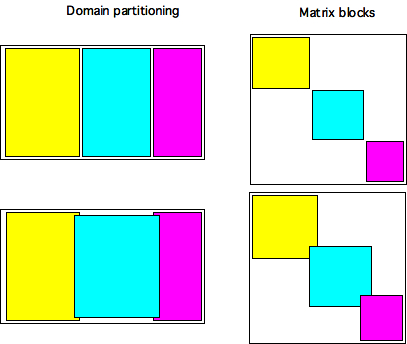
\includegraphics[scale=.5]{bjacobi}
}
\end{higher}

\begin{longversion}
\frame[containsverbatim]{\frametitle{Block Jacobi and Additive Schwarz, theory}
  \begin{itemize}
  \item Both methods parallel
  \item Jacobi fully parallel\\ Schwarz local communication between neighbours
  \item Both require sequential local solver: composition with simple
    precondtitioners
  \item Jacobi limited reduction in iterations\\ Schwarz can be optimal
  \end{itemize}
}

\frame[containsverbatim]{\frametitle{Block Jacobi and Additive Schwarz, coding}

\begin{verbatim}
KSP *ksps; int nlocal,firstlocal; PC pc;
PCBJacobiGetSubKSP(pc,&nlocal,&firstlocal,&ksps);
for (i=0; i<nlocal; i++) {
  KSPSetType( ksps[i], KSPGMRES );
  KSPGetPC( ksps[i], &pc );
  PCSetType( pc, PCILU );
}
\end{verbatim}

Much shorter: commandline options \n{-sub_ksp_type} and \n{-sub_pc_type}
(subksp is PREONLY  by default)

\begin{verbatim}
PCASMSetOverlap(PC pc,int overlap);
\end{verbatim}
}
\end{longversion}

\begin{exerciseframe}[ksp]
  File \n{ksp.c}~/ \n{ksp.F90} contains the solution of a (possibly
  nonsymmetric) linear system.

  Compile the code and run it. Now experiment with commandline
  options. Make notes on your choices and their outcomes.
  \begin{itemize}
  \item The code has two custom commandline switch:
    \begin{itemize}
    \item \n{-n 123} set the domain size to~$123$ and therefore the
      matrix size to~$123^2$.
    \item \n{-unsymmetry 456} adds a convection-like term to the
      matrix, making it unsymmetric. The numerical value is the actual
      element size that is set in the matrix.
    \end{itemize}
  \item What is the default solver in the code? Run with \n{-ksp_view}
  \item Print out the matrix for a small size with \n{-mat_view}.
  \item Now out different solvers for different matrix sizes and
    amounts of unsymmetry. See the instructions in the code.
  \end{itemize}
\end{exerciseframe}

\begin{exerciseframe}[shell]
  After the main program, a routine \n{mymatmult} is
  declared, which is attached by \n{MatShellSetOperation} to the matrix
  \n{A} as the means of computing the product \n{MatMult(A,in,out)}, for
  instance inside an iterative method.

  In addition to the shell matrix \n{A}, the code also creates a
  traditional matrix \n{AA}. Your assignment is to make it so that
  \n{mymatmult} computes the product $y\leftarrow A^tAx$.

  In C, use \n{MatShellSetContext} to attach \n{AA} to \n{A} and
  \n{MatShellGetContext} to retrieve it again for use; in Fortran use a
  common block (or a module) to store \n{AA}.

  The code uses a preconditioner \n{PCNONE}. What happens if you run it
  with option \n{-pc_type jacobi}?
\end{exerciseframe}

\frame[containsverbatim]{\frametitle{Monitors and convergence tests}
\begin{verbatim}
KSPSetTolerances(solver,rtol,atol,dtol,maxit);
\end{verbatim}
Monitors can be set in code, but simple cases:
\begin{itemize}
\item \n{-ksp_monitor}
\item \n{-ksp_monitor_true_residual}
\end{itemize}
}

\begin{longversion}
\frame[containsverbatim]{\frametitle{Custom monitors and convergence tests}
\begin{verbatim}
KSPMonitorSet(KSP ksp,
 PetscErrorCode (*monitor)
      (KSP,PetscInt,PetscReal,void*),
 void *mctx,
 PetscErrorCode (*monitordestroy)(void*));
KSPSetConvergenceTest(KSP ksp,
 PetscErrorCode (*converge)
      (KSP,PetscInt,PetscReal,KSPConvergedReason*,void*),
 void *cctx,
 PetscErrorCode (*destroy)(void*))
\end{verbatim}
}

\frame[containsverbatim]{\frametitle{Example of convergence tests}
\begin{verbatim}
PetscErrorCode resconverge
(KSP solver,PetscInt it,PetscReal res,
 KSPConvergedReason *reason,void *ctx)
{
  MPI_Comm comm; Mat A; Vec X,R; PetscErrorCode ierr;
  PetscFunctionBegin;
  KSPGetOperators(solver,&A,PETSC_NULL,PETSC_NULL);
  PetscObjectGetComm((PetscObject)A,&comm); 
  KSPBuildResidual(solver,PETSC_NULL,PETSC_NULL,&R);
  KSPBuildSolution(solver,PETSC_NULL,&X); 
  /* stuff */
  if (sometest) *reason = 15;
  else *reason = KSP_CONVERGED_ITERATING;
  PetscFunctionReturn(0);
\end{verbatim}
}

%\frame[containsverbatim]{\frametitle{monitors including sing-monitor}
% PetscDrawLG lg;
% KSPMonitorLGCreate(char *display,char *title,int x,int y,int w,int h,PetscDrawLG *lg);
% KSPMonitorSet(KSP ksp,KSPMonitorLG,lg,0);
% When no longer needed, the line graph should be destroyed with the command
% KSPMonitorLGDestroy(PetscDrawLG lg);
% The user can change aspects of the graphs with

% KSPSetComputeEigenvalues(KSP ksp,PETSC TRUE);
% KSPComputeEigenvalues(KSP ksp, int n,double *realpart,double *complexpart,int *neig);
%}

\frame[containsverbatim]{\frametitle{Advanced options}
Many options for the (mathematically) sophisticated user\\
some specific to one method
\begin{verbatim}
KSPSetInitialGuessNonzero
KSPGMRESSetRestart
KSPSetPreconditionerSide
KSPSetNormType
\end{verbatim}
Many options easier through commandline.
}

\frame[containsverbatim]{\frametitle{Null spaces}

\begin{verbatim}
MatNullSpace sp;
MatNullSpaceCreate /* constant vector */
    (PETSC_COMM_WORLD,PETSC_TRUE,0,PETSC_NULL,&sp);
MatNullSpaceCreate /* general vectors */
    (PETSC_COMM_WORLD,PETSC_FALSE,5,vecs,&sp);
KSPSetNullSpace(ksp,sp);
\end{verbatim}

The solver will now properly remove the null space at each iteration.
}
\frame[containsverbatim]{\frametitle{Matrix-free solvers}
Shell matrix requires shell preconditioner
in \n{KSPSetOperators}):
\begin{verbatim}
PCSetType(pc,PCSHELL);
PCShellSetContext(PC pc,void *ctx);
PCShellGetContext(PC pc,void **ctx);
PCShellSetApply(PC pc,
    PetscErrorCode (*apply)(void*,Vec,Vec));
PCShellSetSetUp(PC pc,
    PetscErrorCode (*setup)(void*))
\end{verbatim}
similar idea to shell matrices

Alternative: use different operator for preconditioner
}
\end{longversion}

\begin{shortversion}
  \frame[containsverbatim]{\frametitle{More KSP topics}
  \begin{itemize}
  \item Custom monitors and convergence tests
  \item Method-specific options (especially GMRES)
  \item Null spaces
  \end{itemize}
}
\end{shortversion}

\frame[containsverbatim]{\frametitle{Fieldsplit preconditioners}
If a problem contains multiple physics, seperate preconditioning can
make sense

Matrix block storage: \n{MatCreateNest}
\[ 
\begin{pmatrix}
  A_{00}&A_{01}&A_{02}\\ A_{10}&A_{11}&A_{12}\\ A_{20}&A_{21}&A_{22}\\ 
\end{pmatrix}
\]
However, it makes more sense to interleave these fields
}

\frame[containsverbatim]{
Easy case: all fields are the same size
\begin{verbatim}
PCSetType(prec,PCFIELDSPLIT);
PCFieldSplitSetBlockSize(prec,3);
PCFieldSplitSetType(prec,PC_COMPOSITE_ADDITIVE);
\end{verbatim}
Subpreconditioners can be specified in code, but easier with options:
\begin{verbatim}
PetscOptionsSetValue
 ("-fieldsplit_0_pc_type","lu");
PetscOptionsSetValue
 ("-fieldsplit_0_pc_factor_mat_solver_package","mumps");
\end{verbatim}
Fields can be named instead of numbered.
}

\frame[containsverbatim]{

Non-strided, arbitrary fields: \n{ PCFieldSplitSetIS()}

Stokes equation can be detected:
\n{-pc_fieldsplit_detect_saddle_point}

Combining fields multiplicatively: solve
\[ 
\begin{pmatrix} I\\ A_{10}A_{00}\inv&I \end{pmatrix}
\begin{pmatrix} A_{00}&A_{01}\\ &A_{11} \end{pmatrix}
\]
If there are just two fields, they can be combined by Schur complement
\[ 
\begin{pmatrix} I\\ A_{10}A_{00}\inv&I \end{pmatrix}
\begin{pmatrix} A_{00}&A_{01}\\ &A_{11}-A_{10}A_{00}\inv A_{01} \end{pmatrix}
\]
}

\frame[containsverbatim]{\frametitle{Fieldsplit example}
\begin{verbatim}
 KSPGetPC(solver,&prec);
 PCSetType(prec,PCFIELDSPLIT);
 PCFieldSplitSetBlockSize(prec,2);
 PCFieldSplitSetType(prec,PC_COMPOSITE_ADDITIVE);
 PetscOptionsSetValue
    ("-fieldsplit_0_pc_type","lu");
 PetscOptionsSetValue
    ("-fieldsplit_0_pc_factor_mat_solver_package","mumps");
 PetscOptionsSetValue
    ("-fieldsplit_1_pc_type","lu");
 PetscOptionsSetValue
    ("-fieldsplit_1_pc_factor_mat_solver_package","mumps");
\end{verbatim}
}

\frame[containsverbatim]{\frametitle{Global preconditioners: MG}
\begin{verbatim}
PCSetType(PC pc,PCMG);
PCMGSetLevels(pc,int levels,MPI Comm *comms);
PCMGSetType(PC pc,PCMGType mode);
PCMGSetCycleType(PC pc,PCMGCycleType ctype);
PCMGSetNumberSmoothUp(PC pc,int m);
PCMGSetNumberSmoothDown(PC pc,int n);
PCMGGetCoarseSolve(PC pc,KSP *ksp);
PCMGSetInterpolation(PC pc,int level,Mat P); and
PCMGSetRestriction(PC pc,int level,Mat R);
PCMGSetResidual(PC pc,int level,PetscErrorCode
(*residual)(Mat,Vec,Vec,Vec),Mat mat);
\end{verbatim}
}

\frame[containsverbatim]{\frametitle{Global preconditioners: Hypre}
  \begin{itemize}
  \item Hypre is a package like PETSc
  \item selling point: fancy preconditioners
  \item Install with \n{--with-hypre=yes --download-hypre=yes}
  \item then use \n{-pc_type hypre -pc_hypre_type parasails/boomeramg/euclid/pilut}
  \end{itemize}
  
}

\begin{details}
\frame[containsverbatim]{\frametitle{Direct methods}
  \begin{itemize}
  \item Iterative method with direct solver as preconditioner would
    converge in one step
  \item Direct methods in PETSc implemented as special iterative
    method: \n{KSPPREONLY} only apply preconditioner
  \item All direct methods are preconditioner type \n{PCLU}: 
  \end{itemize}
\begin{verbatim}
myprog -pc_type lu -ksp_type preonly \
    -pc_factor_mat_solver_package mumps 
\end{verbatim}
}
\end{details}

\begin{higher}
\frame[containsverbatim]{\frametitle{Other external PCs}
If installed, other parallel preconditioner are available:

\begin{itemize}
\item
From Hypre: \n{PCHYPRE} with subtypes \n{boomeramg, parasails, euclid, pilut}:\\\n{PCHYPRESetType(pc,parasails)}\\ or \n{-pc_hypre_type parasails}
\item \n{PCSPAI} for Sparse Approximate Inverse
\item \n{PCPROMETHEUS}
\item External packages' existence can be tested:
\begin{verbatim}
%% grep hypre $PETSC_DIR/$PETSC_ARCH/include/petscconf.h
#ifndef PETSC_HAVE_HYPRE
#define PETSC_HAVE_HYPRE 1
#ifndef PETSC_HAVE_LIBHYPRE
#define PETSC_HAVE_LIBHYPRE 1
\end{verbatim}
\end{itemize}
}
\end{higher}

\endinput

\frame[containsverbatim]{\frametitle{Multigrid}
PETSc provides support for three algebraic multigrid codes, all 
parallel. Follow the links from 
http://www-unix.mcs.anl.gov/petsc/petsc-as/documentation/linearsolvertable.html
<http://www-unix.mcs.anl.gov/petsc/petsc-as/documentation/linearsolvertable.html>
under preconditioner, under multigrid under algebraic (ignore the SAMG).

Point-block algebraic multigrid solvers?: you could try Prometheus
(petsc-dev has an interface to it). It was originally designed for
structural analysis problems but has been extended a bit. I don't 
know any others.
- Boomeramg
For BOOMERAMG, PETSc allow me to specify the smoothers as well the
number of pre and post sweeps for fine, coarse, and intermediate levels
of the multigrid cycle by using simple options of the type
\n{'-pc_hypre_boomeramg_XXXX'.
}            - ML
Yes. We only use ML to generate matrices, the prolongation/restriction
operators at all levels. All other operations are carried out
by petsc. Run your code with \n{'-pc_type} ml -help |grep ml '
will show you all options of ml.

My question is then about the appropriate way to specify the smoothers,
number of pre and post sweeps for the different levels of the multigrid
cycle.

Run petsc example ~petsc/src/ksp/ksp/examples/tests/ex26.c
with \n{'-pc_type} ml -help' should give you detailed instructions
on specifying the smoothers.


For example, I want to define a 3-level cycle with :

1 Gauss-Seidel pre-sweep
1 Gauss-Seidel post-sweep
for the fine levels

and 

1 pilut/hypre solve for the coarse level.

Is it then right to use these options

\begin{verbatim}
-pc_type ml
-pc_mg_smoothup 1
-pc_mg_smoothdown 1
-pc_ml_maxNlevels 3

// for the coarse level:
-mg_coarse_ksp_type preonly
-mg_coarse_pc_type hypre
-mg_coarse_pc_hypre_type pilut

// for the fine level:

HERE, I DON'T KNOW HOW TO SPECIFY GAUSS-SEIDEL SWEEPS .....

-mg_levels_pc_type sor
-mg_levels_ksp_type richardson
\end{verbatim}

Note: always makde a test run with \n{-ksp_view} and see
what options it is using, to make sure you set them correctly.

Final note: you can set different otions for different levels
with \n{-mg_levels_1_pc_type ilu -mg_levels_2_pc_type sor}
0 is always the coarsest level.

You can set it for all the levels except the coarse by omitting the
number. \n{-mg_levels_XXXX}
}

\frame[containsverbatim]{\frametitle{Unusual ones:}
- PCFieldSplit
}


